\documentclass{beamer}

\usepackage[utf8]{inputenc}
\usepackage[T1]{fontenc}

\title{MicMac -- un aperçu global}
%\subtitle{Beamer demonstration: longer subtitle}
\institute{IGN}
\date[25 May 2018]{Seminar technique}
\author[E Rupnik]{\texttt{ewelina.rupnik@ign.fr}}
\author[J-M Mueller]{\texttt{ewelina.rupnik@ign.fr}}
\author[M Pierrot-Deseilligny]{\texttt{ewelina.rupnik@ign.fr}}

\usetheme{ign}

\begin{document}


    \begin{frame}[plain]
        \titlepage{}
    \end{frame}

	\tableofcontents
	
%%%%%%%%%%%%%%%%%%%%%%%%%%%%%%%%%%%%%%%%%%%%%%%%%%%% Bilans de la prese
%1/ er: introduction/overview of the processing pipeline    ~3 slides ~3mins
%2/ jmm: tie points extraction
%		+no a priori, extraction algos                      ~2-3      ~3mins
%       +with a priori,                                     ~2-3      ~3mins
%		+reduction algos                                    ~2        ~2mins

%3/ er: image orientation
%       sfm				                                    ~2-3      ~3mins
%       BBA                                                 ~2-3      ~3mins
%       structureless BBA                                   ~2-3      ~3mins
%4/ er: georef                                              ~1-2      ~1mins
	
	
%%%%%%%%%%%%%%%%%%%%%%%%%%%%%%%%%%%%%%%%%%%%%%%%%%%% Introduction        
      \section{Introduction}  
        \subsection*{The processing pipeline}
            \begin{frame}{Overview of the processing pipeline}
                %\framesubtitle{The proof uses \textit{reductio ad absurdum}.}
                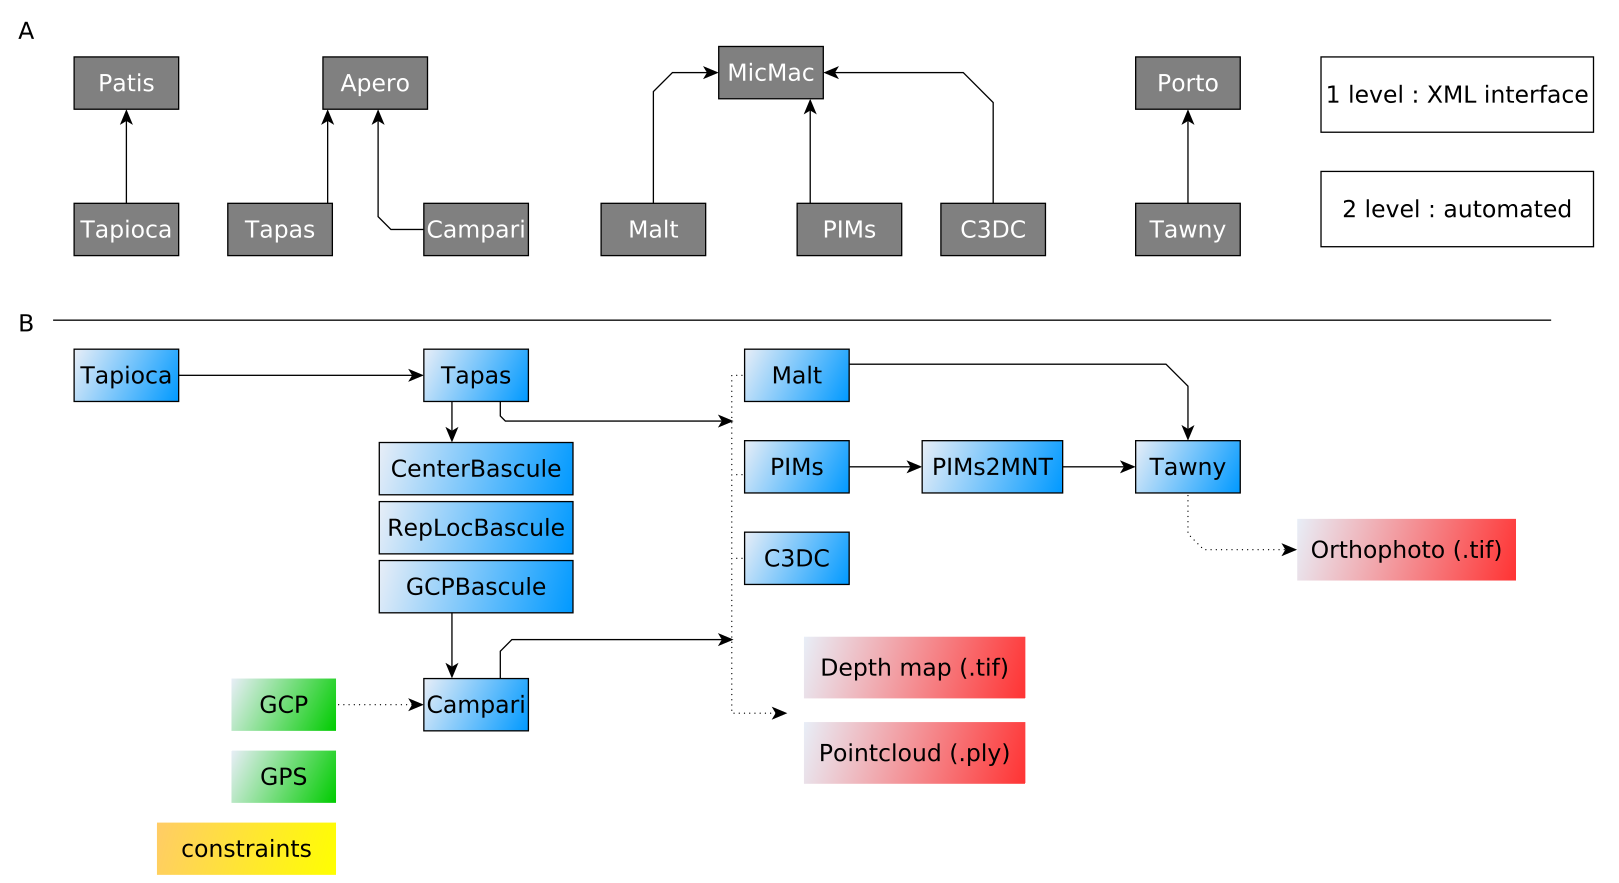
\includegraphics[width=10cm]{images/architecture_prntscr.png}
                
%change the graphic:
% remove A
% add more descriptive names (or maybe in items below Tapas=corresp)                
% introduce tool by tool on diff slides
                
            \end{frame}


%%%%%%%%%%%%%%%%%%%%%%%%%%%%%%%%%%%%%%%%%%%%%%%%%%%% Tie-points
		\section{Tie points extraction}
			\subsection{No {a priori} about the geometry }        
				\begin{frame}{Tie points extraction }
					\framesubtitle{No \textit{a priori} about the geometry}
			
				\begin{block}{Extraction algorithms}
			
				
					\begin{itemize}
					\item SIFT, \\different modes of SIFT (Line, MulScale), i.e. when topology of the acquisition is known (e.g. linear in drone acquisitions or Stereopolosh acquistion)
					\item AIME (presented by MPD during spotlight), under developpment; generally faster than SIFT
					\end{itemize}
 				\end{block}	
					

			
				\end{frame}

			\subsection{With {a priori} about the geometry }        
				\begin{frame}{Tie points extraction }
					\framesubtitle{With \textit{a priori} about the geometry}
					\begin{itemize}
					\item TiePTri
					\end{itemize}
				\end{frame}
        
        	\subsection{Reduction algorithms}
        		\begin{frame}{Tie points reduction algorithms}
        			\begin{itemize}
					\item bla bla
					\end{itemize}
        		\end{frame} 
					
				 
%%%%%%%%%%%%%%%%%%%%%%%%%%%%%%%%%%%%%%%%%%%%%%%%%%%% Pose estimation
\section{Image orientation}       
		\begin{frame}{Image orientation}
			\framesubtitle{Approaches}
			\begin{enumerate}
			\item no a priori, iterative (i.e. SfM)
			\item with a priori, collinearity-based bundle block adjustment (BBA) when initial orientations are known 
			\item structureless BBA
			
			\end{enumerate}
		\end{frame}

	\subsection{SfM}	
		\begin{frame}{SfM}
		
		\end{frame}			

	\subsection{Collinearity-based BBA}	
		\begin{frame}{Collinearity-based BBA}
		
		\end{frame}	

	\subsection{Structureless BBA}	
		\begin{frame}{Structureless BBA}
		
		\end{frame}	
		
%%%%%%%%%%%%%%%%%%%%%%%%%%%%%%%%%%%%%%%%%%%%%%%%%%%% Geo-referencing - maybe put it as a digression next BBA with initial values
\section{Georeferencing}
	\begin{frame}{Georeferencing}
		Mathematical model
		\begin{itemize}
		\item rigid spatial similarity transformation (SST) \\(i.e. 7-param trafo)
		\item "non-rigid" SST (i.e. 7-param and a polynomial)
		\end{itemize}
		
		\onslide<2->Possible input data 
		\begin{enumerate}
			\item<2-> ground control points
			\item<2-> GNSS perspective centers
		\end{enumerate}
	\end{frame}


			
%%%%%%%%%%%%%%%%%%%%%%%%%%%%%%%%%%%%%%%%%%%%%%%%%%%% Ex slide        
%      \section{Ex Slide}  
%        \subsection{slide}
%            \begin{frame}{There Is No Largest Prime Number}
%                \framesubtitle{The proof uses \textit{reductio ad absurdum}.}
%                \begin{theorem}
%                    There is no largest prime number. \end{theorem}
%                \begin{enumerate}
%                    \item<1-| alert@1> Suppose $p$ were the largest prime number.
%                    \item<2-> Let $q$ be the product of the first $p$ numbers.
%                    \item<3-> Then $q+1$ is not divisible by any of them.
%                    \item<1-> But $q + 1$ is greater than $1$, thus divisible by some prime
%                    number not in the first $p$ numbers.
%                \end{enumerate}
%            \end{frame} 
        
\end{document}
